\documentclass[10pt,notoc]{cekarticle}
\usepackage{array}
\usepackage{wrapfig}

\begin{document}

%=============================================================================
% Title page
%=============================================================================

\title{SCHUCS: A UML-Based Approach for Describing\\
  Data Representations Intended for XML Encoding}

\author{Michael Hucka}

\authoremail{mhucka@caltech.edu}

\address{Systems Biology Workbench Development Group\\
  ERATO Kitano Systems Biology Project\\
  Control and Dynamical Systems, MC 107-81\\
  California Institute of Technology, Pasadena, CA 91125}

\acknowledge{Principal Investigators: John Doyle and Hiroaki Kitano}

\date{Version of 11 December 2000}

\maketitlepage

\vspace*{-7pt}


%=============================================================================
\section{Introduction} 
\label{sec:introduction}
%=============================================================================

One component of the ERATO Kitano Systems Biology Project is the creation
of a workbench that provides interoperability between a number of
simulation packages.  Developing a framework for database storage and
inter-program exchange requires defining a language for communicating data.
Defining this language requires first establishing a notation that humans
can use to describe the data structures involved.

I propose a notation to be used for describing data structures that are
intended to be encoded using XML, the Extensible Markup Language~(Bosak and
Bray, 1999; Bray, Paoli and Sperberg-McQueen, 1998; Fallside, 2000).  The
notation is based in part on a subset of UML, the Unified Modeling
Language~(Eriksson, 1998; Oestereich, 1999), a visual language for
specifying software systems.  There are three main advantages to using UML
class diagrams as a basis for defining data structures.  First, compared to
using other notations or a programming language, the UML visual
representations are generally easier to read and understand by readers who
are not computer scientists.  Second, the visual notation is
implementation-neutral---the defined structures can be encoded in any
concrete implementation language, not just XML but other formats as well,
making the UML-based definitions more useful and flexible.  Third, UML is a
de facto industry standard~(OMG, 2000), documented in many books and
available in many software tools including mainstream development
environments (such as Microsoft Visual Basic 5 Enterprise Edition).
Readers are therefore more likely to be familiar with it than other
notations.

Readers do not need to know UML in advance; this document provides
descriptions of all the constructs used.  The notation presented here can
be expressed not only in graphical diagram form (which is what UML is all
about) but also in textual form, allowing descriptions to be easily written
in a text editor and sent as plain-text email.

The scope of the notation is limited to classes and their attributes, not
class methods or operations.  One of the goals of this effort has been to
develop a consistent, systematic method for translating UML-based class
diagrams into XML Schemas.  Another goal has been to maintain a reasonably
simple notation and UML-to-XML mapping.  An important side-effect of this
is that the vocabulary of the notation is purposefully limited to only a
small number of constructs.  It is explicitly \emph{not} intended to cover
the full power of UML or XML.  This limited vocabulary has nevertheless
been sufficient for the applications to which it has been applied so far in
the Systems Biology workbench project.


%=============================================================================
\section{Representing Object Structures in XML}
\label{sec:representing}
%=============================================================================

XML provides the ability to define hierarchically-nested structures; this
works well for representing object-oriented data because objects are
basically nested field-value structures.  An XML data stream or document
consists of a series of descriptions of data objects.  The structure of the
data stream, meaning the permitted vocabulary and organization of entities
in the stream, can be optionally predefined in the form of either a
\emph{Document Type Definition} or an \emph{XML Schema}.

An \emph{XML Schema} (Biron and Malhotra, 2000; Fallside, 2000; Thompson et
al., 2000) is used to specify the kinds of objects allowed in an XML data
stream, as well as how the objects and their properties are to be organized
and the types of values that can be assigned to the object attributes.  It
provides more expressive power than the alternative mechanism for defining
XML structures, the document type definition (DTD).

The following is an example XML Schema definition for a simple kind of data
object:
\begin{example}
<xs:schema xmlns:xs="http://www.w3.org/1999/XMLSchema">

  <xs:complexType name="ObjectClass">
    <xs:attribute name="attributeA" type="xs:string"/>
    <xs:attribute name="attributeB" type="xs:integer"/>
  </xs:complexType>
  
  <xs:element name="Object" type="ObjectClass"/>

</xs:schema>
\end{example}
This definition begins with a qualified element, \verb|xs:schema|, that
tells an XML parser that the rest of the stream is an XML Schema
definition.  The symbols that belong to the XML Schema standard are
prefixed with the characters ``\verb|xs:|''.  The use of \verb|xs:| in
particular, rather than some other prefix, is set by the
\verb|xmlns:xs="..."| portion of the first line.  This is a
\emph{namespace} specification that communicates to the parser that the
prefixed symbols belong to the space of symbols defined for XML Schema.
The rest of the Schema defines an object class unimaginatively called
\verb|ObjectClass| having two attributes \verb|attributeA| and
\verb|attributeB|.  The second-to-last line states that an instance of an
XML data stream based on this Schema definition can contain one top-level
object, called \verb|Object|, constructed according to the class
\verb|ObjectClass|.

Attribute types and other characteristics are defined in the following
sections, along with principles for combining them and defining object
classes.  For brevity, in the rest of this document, only the relevant XML
Schema definitions are given, without enclosing
\verb|<xs:schema ...> ... </xs:schema>| wrappers and without explicit
definition of top-level objects that use the object classes defined.

Although it is extremely powerful, the XML Schema language (and for that
matter, the DTD language) is complicated and not suitable as a descriptive
specification language for humans communicating about data structures used
in a software project.  A more suitable language is UML, but there does not
exist an agreed-upon approach for translating object classes represented in
UML class diagrams into XML Schemas.  The rest of this document presents
one viable approach.

%-----------------------------------------------------------------------------
\subsection{Basis of the Approach}
\label{sec:xml}
%-----------------------------------------------------------------------------

\begin{wrapfigure}[8]{r}{1.5 in}
  \begin{center}
    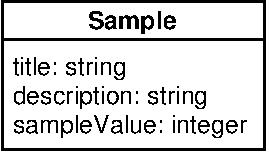
\includegraphics[scale = 0.7]{sampleschema}
  \end{center}
\end{wrapfigure}
An instance of a data object is always constructed according to a blueprint
or \emph{class} definition that specifies the internal structure of the
object.  The ``structure'' is its attributes and the types of data values
that are permitted to be stored in the attributes.  In UML notation, a
class is represented as a box with a title and a list of attributes below
it, as in the example shown at right.  The example shows an object class
named \class{Sample} having three attributes: \attrib{title},
\attrib{description}, and \attrib{sampleValue}.  A full class definition
would also include a list of operations or methods that an object
understands, but the scope of the present effort is limited to data
attributes only.

\newpage

In XML, objects in a document or data stream are referred to as
\emph{elements}.  Elements can contain values that may themselves be other
elements, and elements can have annotations in the form of attributes.  The
following snippet of XML illustrates the different parts of an XML
representation:
\begin{example}
<element1 attributeA="attributeA-value">element1-value</element1>
<element2 attributeB="attributeB-value" attributeC="attributeC-value">
  <element3>element3-value</element3>
  <element4 attributeD="attributeD-value">element4-value</element4>
</element2>
\end{example}
The example above shows four separate elements.  Some of the elements have
attributes (\texttt{element1}, \texttt{element2}, \texttt{element4}), while
others do not (\texttt{element3}).  Some of the elements have simple values
(\texttt{element1}, \texttt{element3}, \texttt{element4}), while the other
one (\texttt{element2}) contains two other elements (\texttt{element3},
\texttt{element4}) as its value.

XML element attributes are name-value pairs that can only be used to hold
simple (scalar) values.  Storing a value that is more structured (e.g.,
another object) requires the use of a subelement.  When encoding a UML data
structure in XML, an attribute in the UML structure may or may not be made
into an XML element attribute.  Indeed, one of the first questions that
needs to be answered when developing an XML format is: what should be
stored as element attributes, and what should be stored as element values?

There is no agreed-upon rule to answer this question.  Some authors lean
towards using element values to store content and attributes to store
annotations about the elements (Box, Skonnard and Lam, 2000; St.~Laurent,
2000).  But this is not universally accepted~(Cover, 2000), and in fact,
one of the original architects of XML has stated that ``I've never heard a
convincing universal decision procedure for what should be an element and
what an attribute''~(Bray, 1998).  Instead of representing data object
attributes as separate XML elements, it is also valid to represent them as
a collection of attributes on a single element.  To put this into concrete
terms, here are two XML samples that can both be taken to express the same
data:
\begin{center}
  \setlength{\tabcolsep}{20 pt}
  \setlength{\extrarowheight}{5pt}
  \tightspacing
  \small
  \vspace*{-\extrarowheight}
  \begin{tabular}{@{}ll@{}}
    \begin{minipage}[t]{1.5 in}
      \begin{tabbing}
        xx\=\kill
        \verb|<Sample>|\\
        \>\verb|<title>My title</title>|\\
        \>\verb|<description>My description</description>|\\
        \>\verb|<sampleValue>42</sampleValue>|\\
        \verb|</Sample>|
      \end{tabbing}
    \end{minipage}
    &
    \begin{minipage}[t]{1.5 in}
      \begin{tabbing}
        xSample \=\kill
        \verb|<Sample title="My title"|\\
                \>\verb|description="My description"|\\
                \>\verb|sampleValue="42"/>|
      \end{tabbing}
    \end{minipage} \\
    \emph{Approach 1} & \emph{Approach 2}
  \end{tabular}
\end{center}
The second approach is a more compact encoding, in part because it can be
written using a short format, \texttt{<tag .../>}, instead of the full
nested tag pair \texttt{<tag ...></tag>}; the shorter format is allowed
when an XML element does not have a value.  The approach also leads to a
direct correspondence between object attributes and XML element attributes:
when we speak about an ``attribute'' of an object, the corresponding XML
construct is usually an attribute on an element, as in the example on the
right above.  For these reasons, the notation presented here is based on
the second approach.

%=============================================================================
\section{The UML-Based Notation and Its Textual and XML Forms}
\label{sec:schemas}
%=============================================================================

The following example presents an object class definition in the UML-style
notation adopted here, along with its representation in a textual form and
in XML Schema syntax:

\begin{center}
  \tightspacing
  \small
  \setlength{\tabcolsep}{6 pt}
  \begin{tabular}{@{}lll@{}}
    \begin{minipage}[b]{1.3 in}
      \raisebox{-2ex}{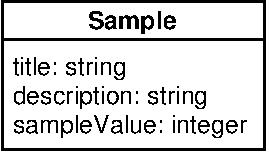
\includegraphics[scale = 0.7]{sampleschema}}
    \end{minipage}
  &
    \begin{minipage}[b]{1.5 in}
      \begin{tabbing}
	sampleValuexx\=\kill
        \class{Sample}\\
	\rule[0.5 ex]{1.3 in}{0.005in}\\
        \attrib{title}:\>\attribtype{string}\\
        \attrib{description}:\>\attribtype{string}\\
        \attrib{sampleValue}:\>\attribtype{integer}
      \end{tabbing}
    \end{minipage}
  &
    \begin{minipage}[b]{3 in}
      \begin{tabbing}
        xx\=\kill
        \verb|<xs:complexType name="Sample">|\\
        \>\verb|<xs:attribute name="title" type="xs:string"/>|\\
        \>\verb|<xs:attribute name="description" type="xs:string"/>|\\
        \>\verb|<xs:attribute name="sampleValue" type="xs:integer"/>|\\
        \verb|</xs:complexType>|
      \end{tabbing}
    \end{minipage}
    \\
    \\
    \emph{UML Form} & \emph{Textual Form} & \emph{XML Schema Form}
  \end{tabular}
  \regularspacing
\end{center}

All three forms define the same data structure: a class \class{Sample} of
objects having three attributes \attrib{title}, \attrib{description} and
\attrib{sampleValue}.  The components are named according to a particular
naming convention.  First, the name of the class must begin with an
uppercase letter, can contain letters, numerals and underscore characters,
and (due to limitations in the software tools we are using) cannot contain
other types of characters.  Words within the names should each be
capitalized.  Second, attribute names generally begin with a lowercase
letter but otherwise follow the convention for class names; for
example, an attribute might be named \attrib{sampleValue}.  An exception to
this rule can be made when the attribute name begins with a word that is
normally capitalized, such as an acronym or symbolic name (e.g.,
``\attrib{Q10Scaling}'').

Attributes are typed.  There are a number of possible datatypes, as
explained in
Sections~\ref{sub:simple-attributes}--\ref{sub:list-attributes}.  The type
specifier is written after the name of the attribute, as in, for example,
\attrib{title:\ string}.  This convention is commonly used in UML textbooks
(e.g., Eriksson and Penker, 1998) and software tools.  An alternative UML
style puts the type specifier before the attribute name, as in, for
instance, \attrib{string title}.

\begin{wrapfigure}[5]{r}{1.4 in}
  \centering
  \raisebox{-2ex}{\includegraphics[scale = 0.7]{sampleschema-abstract}}
\end{wrapfigure}
It is sometimes useful to specify that an object class is \emph{abstract},
meaning that it is only intended to serve as a basis for defining other
classes and not to be instantiated directly into objects.  In such cases,
the class name is written in an italic or slanted typeface, as in the
example shown at right.  In XML, abstract classes are defined by adding
\texttt{abstract="true"} to the type definition:
\begin{example}
<xs:complexType name="Sample" abstract="true">
  ...
</xs:complexType>
\end{example}
To express in the textual form of this notation that a class is abstract,
the name of the class should be followed by the annotation
\class{\{abstract\}} following the name of the class, as in
\class{Sample \{abstract\}}.


%-----------------------------------------------------------------------------
\subsection{Simple Attributes}
\label{sub:simple-attributes}
%-----------------------------------------------------------------------------

\begin{figure}[b]
  \centering
  \small
  \setlength{\tabcolsep}{12 pt}
  \begin{tabular}{@{}ll@{}}
    \raisebox{1.3ex}{
    \begin{minipage}[t]{3in}
      \tightspacing
      \setlength{\tabcolsep}{5 pt}
      \begin{tabular}{@{}ll@{}}
        \textbf{Type} & \textbf{Example(s)} \\
         \hline
         binary		& \texttt{100010} \\
         boolean 	& \texttt{true, false, 1, 0} \\
         byte		& \texttt{-1, 126} \\
         century	& \texttt{19} \\
         date		& \texttt{1999-05-31, ---05} \\
         decimal	& \texttt{-1.23, 0, 123.4, 1000.00} \\
         double		& \texttt{-INF, -0, 0, 1.7E-2, 3, INF, NaN} \\
         ENTITIES \\
         ENTITY \\
         float		& \texttt{-INF, -0, 0, 1.7E-2, 3, INF, NaN} \\
         ID             & \texttt{m32} \\
         IDREF 		& \texttt{m32} \\
         IDREFS         & \texttt{m32 m33 m34 m35} \\
         int		& \texttt{-1, 126789675} \\
         integer	& \texttt{-126789, -1, 0, 1, 126789} \\
         language \\
         long		& \texttt{-1, 12678967543233} \\
         month		& \texttt{1999-05} \\
         Name		& \texttt{shipTo} \\
         NCName		& \texttt{Address} \\
         negativeInteger & \texttt{-126789, -1} \\
       \end{tabular}
       \regularspacing
     \end{minipage}
     }
     &
     \begin{minipage}[t]{3in}
       \tightspacing
       \setlength{\tabcolsep}{5 pt}
       \begin{tabular}{@{}ll@{}}
         \textbf{Type} & \textbf{Example(s)} \\
         \hline
         NMTOKEN 	& \texttt{US} \\
         NMTOKENS	& \texttt{US UK} \\
         nonNegativeInteger	& \texttt{0, 1, 126789} \\
         nonPositiveInteger	& \texttt{-126789, -1, 0} \\
         NOTATION \\
         positiveInteger & \texttt{1, 126789} \\
         QName		& \texttt{po:Address} \\
         recurringDate	& \texttt{--05-31} \\
         recurringDay	& \texttt{----31} \\
         recurringDuration & \texttt{--05-31T13:20:00} \\
         short		& \texttt{-1, 12678} \\
         string		& \texttt{This is a string} \\
         time		& \texttt{13:20:00.000-05}:00 \\
         timeDuration	& \texttt{P1Y2M3DT10H30M12.3S} \\
         timeInstant	& \texttt{1999-05-31T13:20:0.0-05:00} \\
         timePeriod	& \texttt{1999-05-31T13:20} \\
         unsignedByte	& \texttt{0, 126} \\
         unsignedInt	& \texttt{0, 1267896754} \\
         unsignedLong	& \texttt{0, 12678967543233} \\
         unsignedShort	& \texttt{0, 12678} \\
         uriReference	& \texttt{http://www.me.com/x.html\#id5} \\
         year		& \texttt{1999}
       \end{tabular}
       \regularspacing
     \end{minipage}
   \end{tabular}
  \caption{Simple types built into XML Schema, according to the W3C Working
    Draft of 7 April 2000.  Detailed definitions of these types are
    available at \protect\url{http://www.w3.org/TR/xmlschema-2/}.}
  \label{fig:simple-types}
\end{figure}

A simple attribute is one having a simple data value, for instance a number
or a string.  All three of the attributes shown in the \class{Sample}
example above are simple attributes.  The set of simple types that are
permitted is the set defined by the XML Schema Datatypes standard (Biron
and Malhotra, 2000) plus simple types derived from the built-in ones.
Figure~\ref{fig:simple-types} lists the simple types built into XML Schema.

%-----------------------------------------------------------------------------
\subsection{Complex Attributes}
\label{sub:complex-attributes}
%-----------------------------------------------------------------------------

An attribute in an object can be a container for a collection of attributes
under a common heading.  In that case, the attribute is said to be
\emph{complex} because its value is not a simple scalar.  This is roughly
equivalent to a ``struct'' in the language C.

In UML, a complex type is defined as a separate class.  The following is an
example of a class, \class{MyTest}, having three attributes,
\attrib{attributeA}, \attrib{attributeB} and \attrib{attributeC}.  The
first two attributes have simple types, and the third attribute's type is a
newly-defined class, \class{AttrCType}, itself containing two more
attributes.
\begin{quote}
  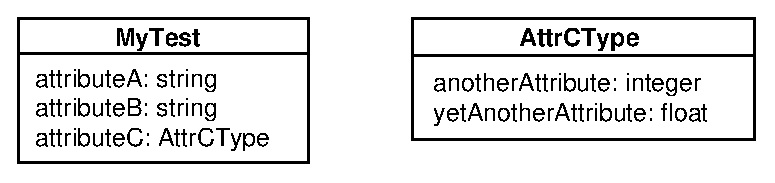
\includegraphics[scale = 0.7]{someschema-uml}
\end{quote}
In a programming language, given an object \texttt{obj} of class
\class{MyTest}, the attributes might be accessed as
\begin{example}
obj.attributeA
obj.attributeB
obj.attributeC.anotherAttribute
obj.attributeC.yetAnotherAttribute
\end{example}

As explained in Section~\ref{sec:xml}, simple attributes in UML class
definitions are translated into element attributes in XML.  Complex types
translate directly into the \attrib{complexType} element in XML Schemas.
However, in XML, an element attribute cannot have a complex type, which
means that a complex attribute in the present notation must be made into an
XML \emph{subelement} within the containing XML element.  This leads to the
question of how to name and structure the subelement.  The approach taken
here is to name the subelement after the attribute, as illustrated in the
following example of an object instance based on \class{MyTest}:
\begin{example}
<MyTest attributeA="foo" attributeB="bar">
  <attributeC anotherAttribute="2" yetAnotherAttribute="4.3"/>
</MyTest>
\end{example}
Note how the attribute \attrib{attributeC} is written out as a separate XML
subelement, but the type of \attrib{attributeC} is not explicitly stated in
the data object.  This is in parallel to how the type also ends up hidden
in the programming language example involving object \verb|obj| given
above.  Only the label \attrib{attributeC} and the attributes
\attrib{anotherAttribute} and \attrib{yetAnotherAttribute} appear.

Here is the XML Schema definition corresponding to the class diagram above:
\begin{exampleTight}
<xs:complexType name="AttrCType">
  <xs:attribute name="anotherAttribute" type="xs:integer"/>
  <xs:attribute name="yetAnotherAttribute" type="xs:float"/>
</xs:complexType>

<xs:complexType name="MyTest">
  <xs:attribute name="attributeA" type="xs:string"/>
  <xs:attribute name="attributeB" type="xs:string"/>
  <xs:element   name="attributeC" type="AttrCType"/>
</xs:complexType>
\end{exampleTight}

%Finally, here is the textual version of the XML Schema above:
%\begin{center}
%  \setlength{\tabcolsep}{20 pt}
%  \tightspacing
%  \small
%  \begin{tabular}{@{}cc@{}}
%    \begin{minipage}{1.6in}
%      \begin{tabbing}
%        AttrCTypexx\=\kill
%        \class{MyClass}\\
%        \rule[0.5 ex]{1.4 in}{0.005in}\\
%        \attrib{attributeA}:\>\attribtype{string}\\
%        \attrib{attributeB}:\>\attribtype{string}\\
%        \attrib{attributeC}:\>\attribtype{AttrCType}
%      \end{tabbing}
%    \end{minipage}
%    & 
%    \begin{minipage}{1.6in}
%      \begin{tabbing}
%        yetanotherattributexxx\=\kill
%        \class{AttrCType}\\
%        \rule[0.5 ex]{1.75 in}{0.005in}\\
%        \attrib{anotherAttribute}:\>\attribtype{integer}\\
%        \attrib{yetAnotherAttribute}:\>\attribtype{float}
%      \end{tabbing}
%    \end{minipage}
%  \end{tabular}
%  \regularspacing
%\end{center}


The only naming convention defined here for complex types is that the names
should begin with a capital letter.  However, it is a good idea to make the
name of a complex type reflect the attribute to which it is connected.
(E.g., for an attribute named \attrib{version}, the complex type might be
named \class{Version}.)

\newpage

%-----------------------------------------------------------------------------
\subsection{Links}
\label{sub:links}
%-----------------------------------------------------------------------------

A link is a reference to another part of the same database object or to a
completely separate database object.  It is a way of referring or pointing
to part of an object, or to a whole other object, by name, without
incorporating the actual physical object itself.  Two different approaches
apply in the two cases, one for intra-object links and one for inter-object
links.  They have parallels in XML, and the present notation reflects the
approach used in XML.

\subsubsection{Intra-Object Links}
\label{subsub:intra}

In XML, links between elements within the same object can be handled
using a particular set of data types that are treated specially by XML
parsers.  The basic idea is the following.  The attribute that contains the
link itself must have the type \class{IDREF}; the referenced component (the
target) must have an attribute of type \class{ID}.  Components of an object
or a particular XML data stream are given unique identifiers assigned to
attributes of type \class{ID}.  Uniqueness of identifiers is enforced by
XML parsers, which are required to collect all attribute values of type
\class{ID} and verify their uniqueness within an XML document or data
stream.  An \class{IDREF} value is required by the XML standard to match
\emph{some} \class{ID} attribute within a given data stream or document, or
else the XML parser must generate an error~(Biron and Malhotra, 2000). The
effect of this is that XML parsers enforce the rule that a link to a
component in an object or data stream does in fact refer to a component
that is actually present.

The type \class{ID} is defined as being a token beginning with a letter or
one of two possible punctuation characters (specifically, underscore or
colon), and continuing with letters, digits, hyphens, underscores, colons,
or full stops, collectively known as \emph{name characters}~(Thompson et
al., 2000).  There is also a list version of \class{IDREF} called
\class{IDREFS} that is not necessary in the present context because of how
lists are handled in this notation; see Section~\ref{sub:list-attributes}.

In order to use this XML facility, the notation described here follows the
XML approach in using attributes of type \class{ID} and \class{IDREF} to
effectuate linking.  The convention adhered to here is that objects that
can be targets of links need to have an attribute named \class{id} of type
\class{ID}.  References to these objects or object components must be made
using attributes of type \class{IDREF}.

The following is a example of a class definition that uses intra-object linking:
\begin{quote}
  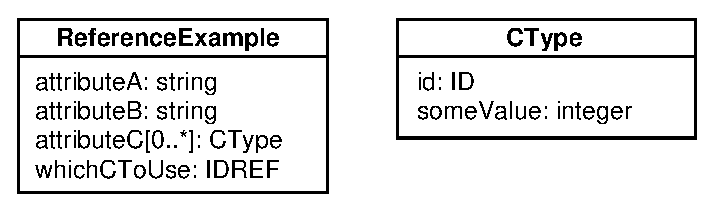
\includegraphics[scale = 0.7]{id-example}
\end{quote}
Here is the XML Schema corresponding to the definition above:
\begin{example}
<xs:complexType name="CType">
  <xs:attribute name="id"        type="xs:ID"/>
  <xs:attribute name="someValue" type="xs:integer"/>
</xs:complexType>

<xs:complexType name="ReferenceExample">
  <xs:attribute name="attributeA" type="xs:string"/>
  <xs:attribute name="attributeB" type="xs:string"/>
  <xs:element   name="listOfAttributeCs">
    <xs:complexType>
      <xs:element name="attributeC" type="CType" minOccurs="0" maxOccurs="unbounded"/>
    </xs:complexType>
  </xs:element>
  <xs:attribute name="whichCToUse" type="xs:IDREF"/>
</xs:complexType>
\end{example}

\newpage

And the following is an example XML stream that makes use of the
definition above:
\begin{example}
<ReferenceExample attributeA="something" attributeB="something else" whichCToUse="c2">
  <listOfAttributeCs> 
    <attributeC id="c1" someValue="42"/>
    <attributeC id="c2" someValue="24"/>
    <attributeC id="c3" someValue="99"/>
  </listOfAttributeCs>
</ReferenceExample>
\end{example}
In the example above, each item in the \attrib{listOfAttributeCs} element
has a different value in the \attrib{id} attribute, and the attribute
\attrib{whichCToUse} refers to one of the items in the list by its
\attrib{id} value.

It is worth noting in passing that this approach can be used to represent
graph structures in XML.  By assigning \class{ID} type identifiers to
different elements in a data structure, it is possible to have elements
link to each other and thereby allow full graph-structured data to be
represented.

\subsubsection{Inter-Object Links}
\label{subsub:inter}

Links may be established between separate objects (i.e., objects in
separate XML data streams or documents).  In UML, a link between two
conceptually separate object classes is indicated by drawing a line between
them.  Such an \emph{association line} can be directed (i.e., an arrow)
when the connection is always from one particular class to the other, and a
third class can be associated with the connection to define additional
properties.  To handle inter-object links in the present framework, all
three of these features need to be invoked.  The following example
illustrates these ideas:
\begin{quote}
  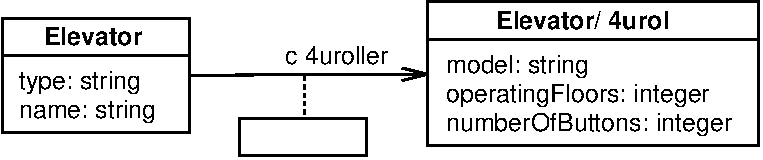
\includegraphics[scale = 0.7]{two-classes}
\end{quote}
The meaning of the above is: \class{Elevator} consists of all the
attributes within the box of the class definition, \emph{plus} the
attribute \attrib{controller}, which is a link of type \class{XLink} to an
object of class \class{ElevatorControl}.  By UML convention, the attribute
\attrib{controller} does not appear in the \class{Elevator} box itself.  In
reading UML diagrams containing associations between classes, it is
therefore important to count \emph{both} the attributes within the class
box as well as the attributes shown on association lines.

Here is the same example in textual form:
\begin{quote}
  \tightspacing
  \small
  \setlength{\tabcolsep}{20 pt}
  \begin{tabular}{@{}ll@{}}
    \begin{minipage}[t]{2.75 in}
      \begin{tabbing}
        controller:xxx\=\kill
        \class{Elevator}\\
	\rule[0.5 ex]{2.75 in}{0.005in}\\
        \attrib{type}:\>\attribtype{string}\\
        \attrib{name}:\>\attribtype{string}\\
        \attrib{controller}:\>\attribtype{XLink  \{link to \class{ElevatorControl}\}}\\
      \end{tabbing}
    \end{minipage}
    &
    \begin{minipage}[t]{1.75 in}
      \begin{tabbing}
        numberOfButtons:xx\=\kill
        \class{ElevatorControl}\\
	\rule[0.5 ex]{1.75 in}{0.005in}\\
        \attrib{model}:\>\attribtype{string}\\
        \attrib{operatingFloors}:\>\attribtype{integer}\\
        \attrib{numberOfButtons}:\>\attribtype{integer}
      \end{tabbing}
    \end{minipage}
  \end{tabular}
\end{quote}
    
A link in the present notation is implemented by using a specific complex
type, \class{XLink}, and then defining attributes that serve as links to be
of this type.  The type \class{XLink} is meant to signify the use of the
\emph{XML Linking Language}, XLink~(DeRose et al., 2000; St. Laurent, 200).
\class{XLink} uses the two essential attributes that define an XML link,
namely \attrib{xlink:type} and \attrib{xlink:href}.  The former can be
given a default value, so only \attrib{xlink:href} needs to be set in
actual use.  The form of the value of the \attrib{xlink:href} reference
target will depend on the particular server storing the database, but the
form will generally be a \class{uriReference} (see
Figure~\ref{fig:simple-types}).  Unfortunately, there is no method for
indicating the intended type of the target object in a simple XLink link;
consistency between the desired type and the actual type of the target
referenced by the link must be handled by the program.

The following XML Schema defines the classes \class{Elevator} and
\class{XLink} used in the example above; the class \class{ElevatorControl}
is assumed to be defined in a separate Schema:
\begin{example}
<xs:complexType name="XLink">
  <xs:attribute name="xlink:type" type="string" use="default" value="simple"/>
  <xs:attribute name="xlink:href" type="xs:uriReference"/>
</xs:complexType>

<xs:complexType name="Elevator">
  <xs:attribute name="type" type="xs:string"/>
  <xs:attribute name="name" type="xs:string"/>
  <xs:element   name="controller" type="XLink"/>
</xs:complexType>
\end{example}
The following is an example of a portion of XML data that uses the Schema:
\begin{example}
<Elevator type="Argo K21" name="Main">
  <controller xlink:href="http://www.myserver.net/db/controllers/kc9"/> 
</Elevator>
\end{example}

For the limited applications that are the domain of the present document,
only the ``simple'' XLink type is required~(DeRose et al., 2000); more
elaborate versions of XLink also exist, but are not used here.


%-----------------------------------------------------------------------------
\subsection{Inclusion}
\label{sub:inclusion}
%-----------------------------------------------------------------------------

The kinds of links described in the previous section point to other
structures without actually including the structures at the point where the
reference occurs.  In some limited situations, it is also useful to include
one data object directly inside another.  For example, programs
communicating data structures in the absence of database facilities may
need to package up entire objects and send them without leaving links that
the recipient may not be able to dereference.  Expressing object inclusion
of this kind requires a variation of the link notation defined in the
previous section.

Inclusion of objects in this fashion is most appropriately handled in XML
using \emph{XInclude}, the XML Inclusions definition~(Marsh and Orchard,
2000).  There are currently significant limitations to using XInclude.  It
is a work in progress and not yet a standard, so the actual syntax of
XInclude described here may vary in the future; moreover, no XML processors
support XInclude yet.  Nevertheless, XInclude is used in the present
notation in anticipation of its eventual standardization.  The XInclude
features used here are extremely limited, so implementing support for
XInclude in application programs should not be difficult.

Here is an example of an object inclusion:
\begin{quote}
  
\includegraphics[scale = 0.7]{xinclude}
\end{quote}

The following XML Schema defines the class \class{Bottle} used in the
example above; the class \class{Brand} is assumed to be defined elsewhere
in a separate Schema:
\begin{example}
<xs:complexType name="XInclude">
  <xs:attribute name="xinclude:href" type="xs:uriReference"/>
</xs:complexType>

<xs:complexType name="Bottle">
  <xs:attribute name="capacity"       type="xs:float"/>
  <xs:attribute name="capacity_units" type="xs:string"/>
  <xs:element   name="brand"          type="XInclude"/>
</xs:complexType>
\end{example}
The following is an example of XML using the Schema:
\begin{example}
<Bottle capacity="5.0" capacity_units="gallon">
  <brand xinclude:href="http://www.myserver.net/bottledb/maker52"/> 
</Bottle>
\end{example}


%-----------------------------------------------------------------------------
\subsection{Lists}
\label{sub:list-attributes}
%-----------------------------------------------------------------------------

An attribute can be a list of simple types, or a list of complex types, or
a list of link or inclusion types.  All items in the list must have the
same type.  In some programming languages such as Java or C, a list might
be represented as a vector or array.

\begin{wrapfigure}[10]{r}{2.2in}
  \begin{center}
    \begin{tabular}{rl}
      1 & exactly one\\
      0,1 & zero or one\\
      0..4 & between zero and four\\
      3,7 & either three or seven\\
      0..* & zero or more\\
      \textrm{*} & zero or more\\
      1..* & one or more
    \end{tabular}
  \end{center}
\end{wrapfigure}
In the diagrammatic and textual forms of the current notation, lists are
expressed using a style loosely based on C and Java-style array notation,
with a multiplicity specifier enclosed in square brackets.  The
\mbox{multiplicity} specifier consists of numerals or the asterisk
character, optionally separated by commas or `..'  (the last to indicate a
range).  Asterisk means ``zero or more''.  For example,
``\attrib{somevar[10]:\ integer}'' means that \attrib{somevar} is a list of
exactly ten integers.  Similarly, ``\attrib{author[1..*]:\ string}'' means
that attribute \attrib{author} is a list of one or more strings.  The table
at the right gives a number of other examples of multiplicity
specifications.

Regardless of whether the type of an attribute is simple, complex, or a
link, the approach used here to translate from a list form into XML is the
same: create a subelement named \class{listOf}\rule{0.5in}{0.5pt}\class{s},
where the blank indicates the capitalized name of the attribute, and then
put a list of elements named after the attribute as the content of the
\class{listOf}\rule{0.5in}{0.5pt}\class{s} element.  Small variations need
to be introduced for coping with various details of different data types,
and these are explained in the following paragraphs.

\subsubsection{Lists of Simple Types}

Perhaps the most natural way of representing a list of simple attributes
would be to have multiple instances of the same attribute on an
object, such as \verb|<Object somevar="value1" somevar="value2" ...>|
However, XML does not allow more than one element attribute of the same
name, therefore an attribute that is a list of simple types must be
translated into a sequence of subelements.  The approach adopted here is to
use a series of subelements named after the attribute, each having a single
element attribute named \attrib{value} used to store the actual value of
the item.  Here is an example:
\begin{quote}
  \tightspacing
  \small
  \setlength{\tabcolsep}{20 pt}
  \begin{tabular}{@{}ll@{}}
    \begin{minipage}[b]{1.5 in}
      \raisebox{-9ex}{\includegraphics[scale = 0.7]{simple-attr-list}}
    \end{minipage}
    & 
    \begin{minipage}[t]{4 in}
\begin{example}
<xs:complexType name="SomeThing">
  <xs:attribute name="attributeA" type="xs:string"/>
  <xs:element   name="listOfAttributeBs">
    <xs:complexType>
      <xs:element name="attributeB" type="xs:string"
                  minOccurs="0" maxOccurs="unbounded"/>
    </xs:complexType>
  </xs:element>
</xs:complexType>
\end{example}
    \end{minipage}
    \\    \\
    \emph{UML Form} & \emph{XML Schema Form}
  \end{tabular}
  \regularspacing
\end{quote}
The definitions above would allow product XML data objects such as the
following; note how the values of the \attrib{attributeB} strings are
recorded on the \attrib{value} attributes in the elements of the list:
\begin{example}
<SomeThing attributeA="123">
  <listOfAttributeBs>
    <attributeB value="first string"/>
    <attributeB value="second string"/>
    <attributeB value="third string"/>
  </listOfAttributeBs>
</SomeThing>
\end{example}


\subsubsection{Lists of Complex Types}

The approach to encoding a complex attribute described in
Section~\ref{sub:complex-attributes} involves translating it into a
subelement.  The approach to encoding a list of complex types parallels the
one for encoding simple types, but without the need for an additional
\attrib{value} attribute.  The elements in the list are each identical to
the element that would be present if there were no list and only a single
complex attribute.  

The following example definition illustrates the idea:
\begin{quote}
  \tightspacing
  \small
  \setlength{\tabcolsep}{20 pt}
  \begin{tabular}{@{}ll@{}}
    \begin{minipage}[b]{1.4 in}
      \raisebox{-23ex}{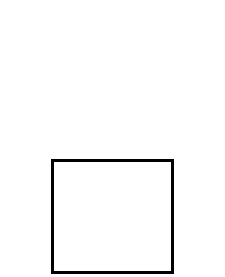
\includegraphics[scale = 0.7]{complex-attr-list}}
    \end{minipage}
    & 
    \begin{minipage}[t]{4 in}
\begin{example}
<xs:complexType name="Point">
  <xs:attribute name="x" type="xs:float"/>
  <xs:attribute name="y" type="xs:float"/>
</xs:complexType>

<xs:complexType name="Triangle">
  <xs:attribute name="name" type="xs:string"/>
  <xs:element   name="listOfPoints">
    <xs:complexType>
      <xs:element name="point" type="Point"
                  minOccurs="0" maxOccurs="unbounded"/>
    </xs:complexType>
  </xs:element>
</xs:complexType>
\end{example}
    \end{minipage}
    \\    \\
    \emph{UML Form} & \emph{XML Schema Form}
  \end{tabular}
  \regularspacing
\end{quote}
The definitions above would allow product XML data objects such as the
following:
\begin{example}
<Triangle name="t1">
  <listOfPoints>
    <point x="2.2" y="1.4"/>
    <point x="0.1" y="4.0"/>
    <point x="0.1" y="1.4"/>
  </listOfPoints>
</Triangle>
\end{example}


\subsubsection{Lists of Links and Inclusions}

The case of intra-object links is identical to the case of a list of simple
attributes discussed above.  Intra-object links
(Section~\ref{subsub:intra}) are implemented simply by using the XML type
\class{IDREF}, so a list of links defined as, for example,
\attrib{itemRef[0..*]:\ IDREF}, turn into a list of elements of the
form \verb|<itemRef value="..."/>|.

In the case of inter-object links or inclusions, multiplicity involving
separate objects is expressed in UML with numerals on the links joining two
object classes together.  For example, if in the \class{Elevator} example
of Section~\ref{sub:links}, \attrib{controller} had actually been a list of
zero or more links to \class{ElevatorControl} class objects, then the
corresponding UML diagram would be:
\begin{quote}
  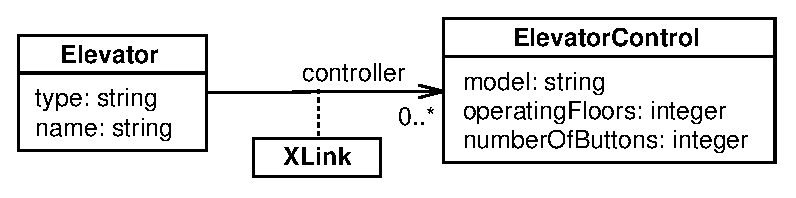
\includegraphics[scale = 0.7]{two-classes-multi}
\end{quote}
By convention, if the relationship is 1-to-1, the two numeral 1's are
normally omitted from the association line in a UML diagram; see the
example diagrams in Sections~\ref{subsub:inter} and \ref{sub:inclusion}.
The absence of any numerals on either end of an association line implies 1.

As in the case of lists of complex types, the elements used in the list of
links or list of inclusions do not need any additional attributes; each
list item has the same form as a single element constructed from a
link attribute as described in Section~\ref{sub:links}.  Here is an example
definition:
\begin{quote}
  \tightspacing
  \small
  \begin{tabular}{@{}ll@{}}
    \begin{minipage}[b]{1.3 in}
      \raisebox{-9ex}{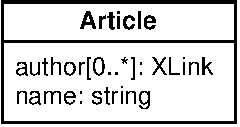
\includegraphics[scale = 0.7]{link-attr-list}}
    \end{minipage}
    & 
    \begin{minipage}[t]{4 in}
\begin{example}
<xs:complexType name="Article">
  <xs:attribute name="name" type="xs:string"/>
  <xs:element   name="listOfAuthors">
    <xs:complexType>
      <xs:element name="author" type="XLink"
                  minOccurs="0" maxOccurs="unbounded"/>
    </xs:complexType>
  </xs:element>
</xs:complexType>
\end{example}
    \end{minipage}
    \\    \\
    \emph{UML Form} & \emph{XML Schema Form}
  \end{tabular}
  \regularspacing
\end{quote}
The following is an XML data object based on the definitions above:
\begin{example}
<Article name="t1">
  <listOfAuthors>
    <author xlink:href="http://www.myserver.net/db/author24"/>
    <author xlink:href="http://www.myserver.net/db/author54"/>
  </listOfPoints>
</Article>
\end{example}

Although the examples above were given in terms of \class{XLink} links, the
same approach also applies to \class{XInclude} inclusions.


%-----------------------------------------------------------------------------
\subsection{Element Values}
%-----------------------------------------------------------------------------

In the present approach to translating UML to XML, most object class
attributes are encoded as attributes on an XML element, and subelements are
likewise used to store information using attributes.  But in addition to
the way that simple and complex types are used here, XML also allows
elements to have content values.  Consider the following example:
\begin{example}
<ContainerExample title="This is a title">
  <bigValue>
    This is some long value, something really long, like a big block
    of text that might be too awkward to put inside an attribute value.
  </bigValue>
</ContainerExample>
\end{example}
The element \attrib{bigValue} above has no attributes, but does have a
value.  Expressing this in UML requires a notation that is not part of UML
proper, so it is necessary to introduce two minor extensions to UML for
this purpose.  The two extensions apply to two different cases:
\begin{enumerate}
  
\item \emph{An attribute representing a container}.  This is the case of
  \class{ContainerExample} illustrated above, where an object's attribute
  is a container for a value in the sense that XML elements can have
  values.  The modified UML notation adopted here is to place the type in
  parentheses.  The parentheses signify that the attribute is special, with
  not actually represented as an attribute in XML but rather as an element
  whose value is significant.  Here follows the definition corresponding to
  the example given above:
  \begin{quote}
    \tightspacing
    \small
    \setlength{\tabcolsep}{10 pt}
    \begin{tabular}{@{}ll@{}}
      \begin{minipage}[b]{1.3 in}
        \begin{center}
          \raisebox{-9ex}{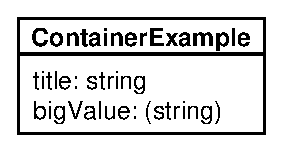
\includegraphics[scale = 0.7]{attribute-container}}
        \end{center}
      \end{minipage}
      & 
      \begin{minipage}[t]{3.75 in}
\begin{example}
<xs:complexType name="ContainerExample">
  <xs:attribute name="title" type="xs:string"/>
  <xs:element   name="bigValue" type="xs:string"/>
</xs:complexType>
\end{example}
      \end{minipage}
      \\    \\
      \emph{UML Form} & \emph{XML Schema Form}
    \end{tabular}
    \regularspacing
  \end{quote}
  Restriction: The type of the container attribute in the definition must
  be simple; it cannot be another a complex type.  (If the type were
  allowed to be complex, the situation would simply be identical to an
  ordinary complex attribute.)
  
\item \emph{A class containing a value}.  For this case, the modified UML notation
  adopted here is to place the type of the container in parentheses
  following the class name.  For example,
  \begin{quote}
    \tightspacing
    \small
    \setlength{\tabcolsep}{10 pt}
    \begin{tabular}{@{}ll@{}}
      \begin{minipage}[b]{1.3 in}
        \begin{center}
          \raisebox{-7ex}{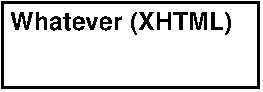
\includegraphics[scale = 0.7]{class-container}}
        \end{center}
      \end{minipage}
      & 
      \begin{minipage}[t]{4 in}
\begin{example}
<xs:complexType name="Whatever" content="textOnly">
  <xs:attribute name="bigDeal" type="xs:string"/>
  <xs:attribute name="type" use="fixed" value="XHTML"/>
</xs:complexType>
\end{example}
      \end{minipage}
      \\    \\
      \emph{UML Form} & \emph{XML Schema Form}
    \end{tabular}
    \regularspacing
  \end{quote}
  This allows the following kind of XML data object:
\begin{example}
<Whatever bigDeal="This is an attribute">
  This has a value, but no subelements.
</Whatever>
\end{example}
  The XML Schema for this case uses the special property
  \attrib{content="textOnly"}, which indicates that the XML element value
  can only contain data, not subelements.  This unfortunately imposes a
  limitation on the resulting representation: XML parsers will not check
  the datatype of the content in instance objects, treating it simply as
  text.  In order to avoid losing the type information altogether, the
  original type is recorded on an attribute called \attrib{type}, using a
  fixed value corresponding to the type stated in parentheses next to the
  class definition.  Although XML parsers will not check the content in
  instance objects, programs that receive objects of this class can use the
  type information to perform their own checking.
  
  Restrictions: (1) The type of the container attribute must be a
  simple type; it cannot be a complex type.  (2) None of the
  attributes in the rest of the object class definition can be complex; all
  must have simple types.


\end{enumerate}  


%-----------------------------------------------------------------------------
\subsection{Constraints on Attribute Values}
%-----------------------------------------------------------------------------

It is important to be able to express constraints on the values of
attributes.  A constraint refers to a limitation or restriction on the
possible content or state of an attribute.  For example, it may be useful
to specify that a given integer attribute cannot have a value less than
zero, or that a given string attribute can only take on values from a
limited vocabulary.

There are two standard ways in UML to express constraints.  One approach
consists of adding a constraint expression in curly braces following the
definition of an attribute, as in the UML shown in the following example:
\begin{quote}
  \setlength{\tabcolsep}{20 pt}
  \tightspacing
  \small
  \begin{tabular}{@{}cc@{}}
    \begin{minipage}[b]{2 in}
      \begin{tabbing}
        attrBxx\=integerxx\=\kill
        \class{AnExample}\\
        \rule[0.5 ex]{2.5 in}{0.005in}\\
        \attrib{attrA}:\>\attribtype{integer}\\
        \attrib{attrB}:\>\attribtype{string}\>\attrib{\{"val1", "val2", "val3"\}}\\
      \end{tabbing}
      \emph{Textual form}
    \end{minipage}
  &
    \begin{minipage}[b]{3 in}
      \raisebox{1ex}{
\includegraphics[scale = 0.7]{someschema-constraints}}\\
      \emph{UML form}
    \end{minipage}
  \end{tabular}
  \regularspacing
\end{quote}
Alternatively, in a UML diagram, the constraints can be placed in an
external text box and a line can be drawn from the box to the attribute in
question, as in the following:
\begin{quote}
  \includegraphics[scale = 0.7]{someschema-constraints-boxed}
\end{quote}

For defining constraints in UML, some authors use Object Constraint
Language, a declarative language based on set theory~(Oestereich, 1999).
For the goals of the present notation, it is more convenient to express
constraints either in a simple stylized form (as in the
immediately-preceding examples) or using XML Schema language.  The
following are some examples that have arisen in practice:
\begin{itemize}
  
\item \emph{String value chosen from a strictly limited vocabulary}.  XML
  Schema defines several mechanisms for constraining values of attributes.
  A particularly useful one is the \attrib{enumeration} component.  Here is
  an example of an XML Schema constraining the values of an attribute to a
  limited set of three specific strings for the class \class{AnExample}
  defined above:
\begin{example}
<xs:complexType name="AnExample">
  <xs:attribute name="attrA" type="xs:integer"/>
  <xs:attribute name="attrB">
    <xs:simpleType base="xs:string">
      <xs:enumeration value="val1"/>
      <xs:enumeration value="val2"/>
      <xs:enumeration value="val3"/>
    </xs:simpleType>
  </xs:attribute>
</xs:complexType>
\end{example}

\item \emph{Optional attribute}.  Sometimes an attribute in a class should
  be considered optional.  For these situations, the attribute should be
  given the XML Schema property \attrib{minOccurs="0"}.  (The default value
  of \attrib{minOccurs} is 1.)
  \begin{quote}
    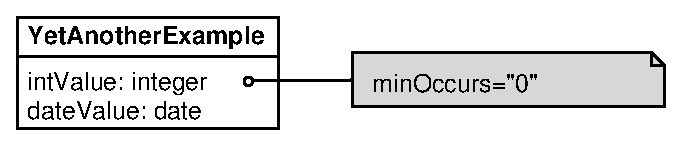
\includegraphics[scale = 0.7]{minoccurs}
  \end{quote}
  \emph{UML Form}
\begin{example}
<xs:complexType name="YetAnotherExample">
  <xs:attribute name="intValue"  type="xs:integer" minOccurs="0"/>
  <xs:attribute name="dateValue" type="xs:date"/>
</xs:complexType>
\end{example}
  \emph{XML Schema Form}

\item \emph{Minimum and maximum range values on numeric attributes}.  The
  upper and lower value boundaries for an attribute having a numeric value
  can be defined using the XML Schema \attrib{minExclusive},
  \attrib{minInclusive}, \attrib{maxInclusive}, and \attrib{maxExclusive}
  properties.  For instance:

    \vspace*{1ex}
  \begin{quote}
    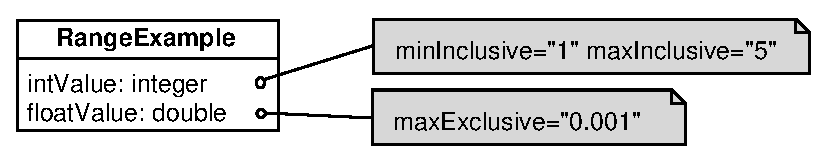
\includegraphics[scale = 0.7]{min-max}
  \end{quote}
  \emph{UML Form}
\begin{example}
<xs:complexType name="RangeExample">
  <xs:attribute name="intValue"   type="xs:integer" minInclusive="1" maxInclusive="10"/>
  <xs:attribute name="floatValue" type="xs:double"  maxExclusive="0.001"/>
</xs:complexType>
\end{example}
  \emph{XML Schema Form}

  The first attribute is limited to integer values from 1 to 10,
  inclusive; the second attribute is constrained to values no less than
  0.001, exclusive.

\end{itemize}

There are many more situations that call for the use of constraints and
that are not covered by the examples above.  For such other cases, it is up
to users of the present notation to devise appropriate expressions of
constraints using XML Schema terms or other simple expressions.  The
constraint terms available in XML Schema are defined in the XML Schema
specification~(Biron and Malhotra, 2000; Thompson et al. 2000).


%-----------------------------------------------------------------------------
\subsection{Specifying Units}
%-----------------------------------------------------------------------------

It is often important to provide information about the units associated
with a numerical attribute.  In the approach to XML representations used
here, there are two alternatives for specifying units conveniently.

The first approach is to define, for each relevant attribute, another
attribute whose name has the suffix \attrib{\_units} and whose type is a
string, to represent the units being used for the value stored in the
attribute.  The following is an example:
\begin{quote}
  \tightspacing
  \small
  \setlength{\tabcolsep}{20 pt}
  \begin{tabular}{@{}ll@{}}
    \begin{minipage}[b]{1.7 in}
      \raisebox{-2ex}{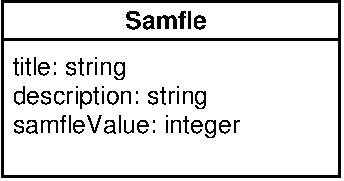
\includegraphics[scale = 0.7]{sampleschema-units}}
    \end{minipage}
  &
    \begin{minipage}[b]{3.2 in}
      \begin{tabbing}
        xx\=\kill
        \verb|<xs:complexType name="Sample">|\\
        \>\verb|<xs:attribute name="title" type="xs:string"/>|\\
        \>\verb|<xs:attribute name="description" type="xs:string"/>|\\
        \>\verb|<xs:attribute name="sampleValue" type="xs:integer"/>|\\
        \>\verb|<xs:attribute name="sampleValue_units" type="xs:string"/>|\\
        \verb|</xs:complexType>|
      \end{tabbing}
    \end{minipage}
    \\
    \\
    \emph{UML Form} & \emph{XML Schema}
  \end{tabular}
  \regularspacing
\end{quote}

The second approach is suitable for groups of attributes or substructures
that all use the same unit.  In that case, it may be simpler to define an
attribute at the class level that sets the units for a whole object.

In order to maximize the utility of having unit specifications, a given
project should define a specific XML type for the units it needs to use.
This specification should take the form of a datatype (perhaps called
\class{Units}), defined in a separate XML Schema, consisting of an
enumeration of strings.  Here is a partial example of such an XML Schema:
\begin{example}
<xs:simpleType name="Units" base="xs:string">
  <xs:enumeration value="m"/>
  <xs:enumeration value="cm"/>
  <xs:enumeration value="mm"/>

  <!-- and so on ... -->

</xs:simpleType>
\end{example}

%-----------------------------------------------------------------------------
\subsection{Inheritance}
%-----------------------------------------------------------------------------

Inheritance allows an object class to be defined as an extension or
derivation of another class.  In textual form, the inheritance relationship
can be written on the same line as the name of the class definition; in
graphical UML form, inheritance is expressed using an open-ended arrow
drawn from an inheriting class to the inherited-from class.  The following
illustrates both forms:

\begin{quote}
  \tightspacing
  \small
  \setlength{\tabcolsep}{30 pt}
  \begin{tabular}{@{}ll@{}}
    \begin{minipage}[b]{1.6in}
      \begin{tabbing}
        Stringxxx\=attrbxxx\=\kill
        \class{SomeOtherClass}\\
        \rule[0.5 ex]{1 in}{0.005in}\\
        \attrib{myValue}:\>\attribtype{string}
      \end{tabbing}
      \vspace*{5pt}
      \begin{tabbing}
        Stringxxx\=attrbxxx\=\kill
        \class{SomeClass extends SomeOtherClass}\\
        \rule[0.5 ex]{2 in}{0.005in}\\
        \attrib{attrA}:\>\attribtype{string}
      \end{tabbing}
    \end{minipage}
    & 
    \begin{minipage}[b]{2 in}
      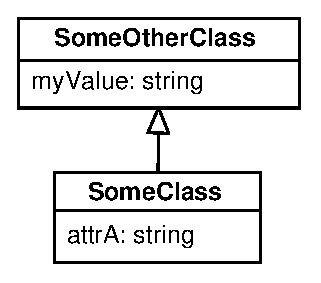
\includegraphics[scale = 0.7]{someschema-inherit}
    \end{minipage} \\ \\
    \emph{Textual form} & \emph{UML form}
  \end{tabular}
  \regularspacing
\end{quote}

The meaning of the above is that \class{SomeClass} inherits from
\class{SomeOtherClass} and augments the latter type's definition by adding
an attribute of its own.  \class{SomeClass} therefore has as attributes
\emph{both} \attrib{attrA} and \attrib{myValue}, even though the box
defining \class{SomeClass} itself does not mention the second one.
\class{SomeOtherClass} has only one attribute, \attrib{myValue}.

In XML, inheritance can be implemented using the \attrib{base} and
\attrib{derivedBy} mechanisms on a type definition.  This allows an XML
element/class definition to be based on another element.  The following is
an XML Schema for the example above:
\begin{example}
<xs:complexType name="SomeOtherClass">
  <xs:attribute name="myValue" type="xs:string"/>
</xs:complexType>

<xs:complexType name="SomeClass" base="SomeOtherClass" derivedBy="extension">
  <xs:attribute name="attrA" type="xs:string"/>
</xs:complexType>
\end{example}


%=============================================================================
\section{Summary}
%=============================================================================

The notation proposed in this document is based on a subset of what could
be used and what UML provides.  It is not intended to cover the full scope
of UML or XML.  The subset was chosen to be as simple as possible yet allow
the expression of the kinds of data structures that need to be encoded in
XML for the ERATO Kitano Systems Biology workbench.

The notation proposed here is not carved in stone, and will undoubtedly
continue to evolve.  Please send your feedback about any aspect of this
document to the author.

%=============================================================================
\section{Acknowledgements}
%=============================================================================

This notation was developed as a result of joint work between fellow
members of the Caltech ERATO Kitano Systems Biology team (Herbert Sauro,
Andrew Finney, Hamid Bolouri) and the Modeler's Workspace project (Kavita
Shankar, David Beeman, Sara Emardson).  I thank Greg Hood, Fred Howel and
Nigel Goddard for additional comments on early versions of this notation.

This research has been supported by a grant from the NIMH Human Brain
Project, an Academic Equipment Grant (\#EDUD-7824-000127-US) from Sun
Microsystems, Inc., and a gift from the Microsoft Corporation.

\appendix


%=============================================================================
\setcounter{secnumdepth}{-1}
\section{References}
%=============================================================================

\setlength{\parskip}{1.2ex}

\begin{flushleft}

Biron, P.~V., and Malhotra, A.  (2000).  XML Schema Part 2: Datatypes (W3C
Working Draft 7 April 2000).  Available via the World Wide Web at
\url{http://www.w3.org/TR/xmlschema-2/}.

Bosak, J., and Bray, T. (1999).  {XML} and the Second-Generation Web.
Scientific American, May.  Also available via the World Wide Web at
\url{http://www.sciam.com/1999/0599issue/0599bosak.html}.

Box, D., Skonnard, A., and Lam, J.  (2000).  \emph{Essential XML}.  Boston:
Addison-Wesley.

Bray, T. (2000).  RE: When is an attribute an attribute?  Posting to the
\url{xml-dev} mailing list, Apr 1998.  Available via the World Wide Web at
\url{http://www.oasis-open.org/cover/brayAttr980409.html}.

Bray, T., Paoli, J., and Sperberg-McQueen, C.~M. (1998). Extensible Markup
Language (XML) 1.0, W3C Recommendation 10-February-1998.  Available via the
World Wide Web at \url{http://www.w3.org/TR/1998/REC-xml-19980210}.

Cover, R.  (2000).  SGML/XML Elements versus Attributes: When Should I Use
Elements, and When Should I Use Attributes?   Available via the World Wide
Web at \url{http://www.oasis-open.org/cover/elementsAndAttrs.html}.

DeRose, S., Maler, E., Orchard, D., and Trafford, B. (2000).  XML Linking
Language (XLink) Version 1.0 W3C Candidate Recommendation 3 July 2000.
Available via the World Wide Web at \url{http://www.w3.org/TR/xlink/}.

Eriksson, H.-E., and Penker, M. (1998).  \emph{UML Toolkit}.  New York: John Wiley
\& Sons.

Fallside, D.~C.  (2000).  XML Schema Part 0: Primer (W3C Working Draft, 7
April 2000).  Available via the World Wide Web at
\url{http://www.w3.org/TR/xmlschema-0/}.

Marsh, J., and Orchard, D.  (2000).  XML Inclusions (XInclude) Version 1.0
(W3C Working Draft 17-July-2000).  Available via the World Wide Web at
\url{http://www.w3.org/TR/xinclude}.

OMG (Object Management Group), (2000).  UML Resource Page.  Available via
the World Wide Web at \url{http://www.omg.org/technology/uml/}.

Oestereich, B.  (1999).  \emph{Developing Software with UML: Object-Oriented
Analysis and Design in Practice}.  Addison-Wesley.

St. Laurent, S. (2000).  \emph{XML Elements of Style}.   New York: McGraw-Hill.

Thompson, H.~S., Beech, D., Maloney, M., and Mendelsohn, N. (2000).  XML
Schema Part 1: Structures (W3C Working Draft 7 April 2000).  Available via
the World Wide Web at \url{http://www.w3.org/TR/xmlschema-1/}.

\end{flushleft}

\end{document}









%XML, the Extensible Markup Language (Bosak and Bray, 1999; Bray, Paoli and
%Sperberg-McQueen, 1998) is a language used to express self-describing,
%structured representations of information.  It provides a way of marking up
%data with semantic tags that describe and structure the contents of the
%data.  Although XML is typically thought of as a document format similar to
%HTML, in fact it is more general.  It is a notation, a ``metalanguage'', a
%way of organizing a stream of data and marking up the different parts so
%that a program can parse the stream into constituents.  In the words of one
%of its chief architects, ``Just as HTML created a way for every computer
%user to read Internet documents, XML makes it possible, despite the Babel
%of incompatible computer systems, to create an Esperanto that all can read
%and write.  Unlike most computer data formats, XML markup also makes sense
%to humans, because it consists of nothing more than ordinary text''~(Bosak
%and Bray, 1999).



%UML notation does not make a clear distinction between a pointer to an
%instance, and actual incorporation of the instance into an object.  To make
%this clear in the presentation notation, we take the approach of defining a
%new class for each link type.  The naming convention is to name the link
%type according to the pattern \class{LinkTo}\rule{0.75in}{0.5pt}, where the
%blank is replaced by the name of the object class.  For example, a link to
%a \class{CellModel} object would be implemented using a type called
%\class{LinkToCellModel}.


%When translating the UML-based notation into XML, the implementation of a
%\class{LinkTo}\rule{0.75in}{0.5pt} type must use XLink syntax.  Although it
%is not possible to define all possible link types here---the list of
%possible types depends on the specific types defined in a particular
%application---the following example XML Schema should give a sense for the
%approach:
%\begin{quote}
%  \begin{small}
%    \tightspacing
%\begin{example}
%<xs:schema xmlns:xs="http://www.w3.org/1999/XMLSchema"
%            xmlns:xlink="http://www.w3.org/2000/xlink">
  
%  <xs:complexType name="LinkToAuthor">
%    <xs:attribute name="xlink:type" type="string" value="simple" use="default"/>
%    <xs:attribute name="xlink:href" type="string"/>
%  </xs:complexType>
  
%  <xs:complexType name="SomeClass">
  
%    <!-- ... other definitions presumably go here ...>
  
%    <xs:element   name="authors" minOccurs="1" maxOccurs="1">
%      <xs:complexType>
%        <xs:element name="LinkToAuthor" type="LinkToAuthor" minOccurs="0" maxOccurs="*"/>
%      </xs:complexType>
%    </xs:element>
  
%    <!-- ... other definitions presumably go here ...>

%  </xs:complexType>

%</xs:schema>
%\end{example}
%    \regularspacing
%  \end{small}
%\end{quote}



%To get a sense for what an actual object might look like, suppose there
%exists an instance of a \class{MyClass} object that has three elements in
%\attrib{attributeC}.  Written in a C or Java-like programming language,
%this might look like the following:
%\begin{quote}
%  \begin{small}
%    \tightspacing
%\begin{example}
%obj.attributeA                        = "foo";
%obj.attributeB                        = "bar";

%obj.attributeC[0].anotherAttribute    = 1;
%obj.attributeC[0].yetAnotherAttribute = 2.2;

%obj.attributeC[1].anotherAttribute    = 5;
%obj.attributeC[1].yetAnotherAttribute = 12.0;

%obj.attributeC[2].anotherAttribute    = 30;
%obj.attributeC[2].yetAnotherAttribute = 40.23;
%\end{example}
%    \regularspacing
%  \end{small}
%\end{quote}
%And now, the same object encoded in XML:
%\begin{quote}
%  \begin{small}
%    \tightspacing
%\begin{example}
%...
%<MyClass attributeA="foo" attributeB="bar">
%  <attributeC>
%    <AttrCType anotherAttribute="1" yetAnotherAttribute="2.2"/>
%    <AttrCType anotherAttribute="5" yetAnotherAttribute="12.0"/>
%    <AttrCType anotherAttribute="30" yetAnotherAttribute="40.23"/>
%  </attributeC>
%</MyClass>
%...
%\end{example}
%  \regularspacing
%\end{small}
%\end{quote}



%One situation arises frequently in data representations, and that is the
%need to constrain the values of a string attribute to be taken from a
%partially or fully constrained vocabulary.  We use the following notation
%to express different kinds of constraints in this context:
%\begin{itemize}
  
%\item If a string attribute's value should be a single string chosen only
%  from a strictly limited vocabulary (known as a controlled vocabulary),
%  the possible values are listed in curly braces next to the attribute:
%  \begin{quote}
%    \small
%    \tightspacing
%    \begin{tabbing}
%      Stringxxx\=attrbxxx\=\kill
%      \class{SomeSchema}\\
%      \rule[0.5 ex]{2.85 in}{0.005in}\\
%      \attrib{attrA}:\>\attribtype{String}\>\attrib{\{``val1'', ``val2'', ``val3''\}}
%    \end{tabbing}
%    \regularspacing
%  \end{quote}
  
%\item If a string attribute's value can be any single string, but the user
%  is to be provided with a list of suggested preferred values (i.e., the
%  vocabulary is partially controlled), the known preferred values are
%  listed in curly braces and an asterisk character is added at the end of
%  the list to indicate any other value is permitted as well:
%  \begin{quote}
%    \small
%    \tightspacing
%    \begin{tabbing}
%      Stringxxx\=attrbxxx\=\kill
%      \class{SomeSchema}\\
%      \rule[0.5 ex]{3.25 in}{0.005in}\\
%      \attrib{attrA}:\>\attribtype{String}\>\attrib{\{``val1'', ``val2'', ``val3'', *\}}
%    \end{tabbing}
%    \regularspacing
%  \end{quote}
  
%\item If a string attribute's value can be one or more strings chosen from
%  either a controlled vocabulary or a partially controlled vocabulary, the
%  constraint is expressed as follows:
%  \begin{quote}
%    \small
%    \tightspacing
%    \begin{tabbing}
%      Stringxxx\=attrbxxx\=\kill
%      \class{SomeSchema}\\
%      \rule[0.5 ex]{4.5 in}{0.005in}\\
%      \attrib{attrA}:\>\attribtype{String}\>\attrib{\{one or more of: ``val1'', ``val2'', ``val3''\}}\\
%      \attrib{attrB}:\>\attribtype{String}\>\attrib{\{one or more of: ``valA'', ``valB'', ``valC'', *\}}
%    \end{tabbing}
%    \regularspacing
%  \end{quote}
%  This particular form (the use of the string ``one or more of'') is not
%  defined in UML; it is a simple extension introduced as part of the
%  notation being described here.

%\end{itemize}
